\subsection{LLM ablation: tools versus advice}
\begin{table*}[t]
\caption{LLM ablation ($2\times2$, two trials per cell, one batch): recovered/trials, median recovery in
seconds (range). Bold: fastest full recovery per fault among the four variants.}
\label{tab:ablation}
\centering
\small
\begin{tabular}{@{}lcccc@{}}
\toprule
 & \multicolumn{2}{c}{No tools} & \multicolumn{2}{c}{Tools (agent)} \\
\cmidrule(lr){2-3}\cmidrule(lr){4-5}
Failure & no guid. & guidance & no guid. & guidance \\
\midrule
\texttt{redis\_down} & 2/2, 4.1\,{\scriptsize(4.0--4.2)} & \textbf{2/2, 3.1\,{\scriptsize(3.0--3.2)}} & 2/2, 15.6\,{\scriptsize(11.4--19.8)} & 2/2, 8.1\,{\scriptsize(6.9--9.2)} \\
\texttt{redis\_latency} & 2/2, 50.1\,{\scriptsize(50.0--50.2)} & \textbf{2/2, 3.3\,{\scriptsize(3.1--3.5)}} & 2/2, 58.6\,{\scriptsize(58.5--58.7)} & 2/2, 8.0\,{\scriptsize(7.7--8.3)} \\
\texttt{postgres\_latency} & $\times$ 0/2 & $\times$ 0/2 & $\times$ 0/2 & $\times$ 0/2 \\
\texttt{postgres\_down} & \textbf{2/2, 7.6\,{\scriptsize(7.2--8.0)}} & $\times$ 0/2 & 2/2, 17.1\,{\scriptsize(12.5--21.6)} & 2/2, 18.9\,{\scriptsize(15.4--22.4)} \\
\texttt{api\_crash} & \textbf{2/2, 13.2\,{\scriptsize(12.8--13.5)}} & 2/2, 44.1\,{\scriptsize(42.6--45.5)} & 2/2, 23.5\,{\scriptsize(23.2--23.7)} & 2/2, 22.1\,{\scriptsize(21.0--23.3)} \\
\midrule
\texttt{redis\_partition} & 2/2, 43.0\,{\scriptsize(42.5--43.5)} & \textbf{2/2, 2.3} & 2/2, 51.1\,{\scriptsize(50.9--51.3)} & 2/2, 28.0\,{\scriptsize(6.5--49.5)} \\
\texttt{redis\_down\_slow\_db} & $\times$ 0/2 & $\times$ 0/2 & $\times$ 0/2 & $\times$ 0/2 \\
\midrule
\textit{recovered} & 10/14 & 8/14 & 10/14 & 10/14 \\
\bottomrule
\end{tabular}
\end{table*}

\begin{figure}[t]
\centering
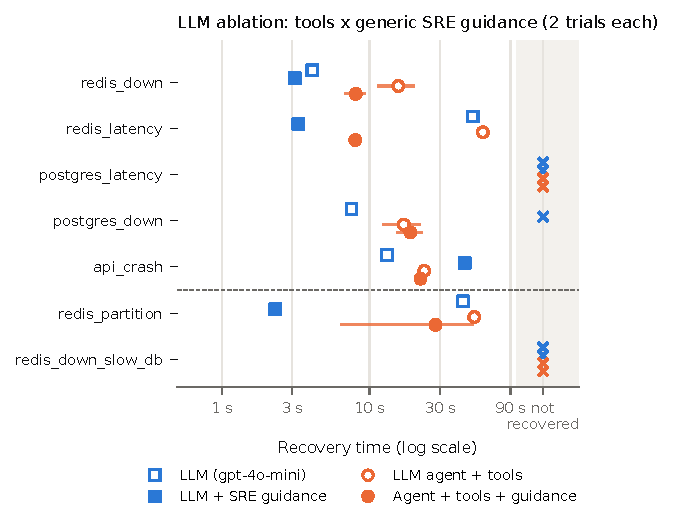
\includegraphics[width=\columnwidth]{fig_ablation.pdf}
\caption{LLM ablation. Squares: no tools; circles: tool-using agent. Hollow: no guidance; filled:
generic SRE guidance. Median recovery (range); $\times$: not recovered.}
\label{fig:ablation}
\end{figure}

Table~\ref{tab:ablation} and Fig.~\ref{fig:ablation} separate the two factors.
\emph{Advice changes the prior.} Without guidance, both LLM variants restarted first on every Redis fault,
which cost 43--59\,s on the two faults a restart cannot fix (\act{redis\_latency}, \act{redis\_partition}).
With the SRE paragraph and no tools, the model chose \act{cache\_bypass} first in \emph{all} 14 of its
trials. This was the fastest LLM behaviour in the study where bypass is right (\act{redis\_latency}
50.1\,s $\rightarrow$ 3.3\,s, \act{redis\_partition} 43.0\,s $\rightarrow$ 2.3\,s, medians) and harmful
where a restart is right: it never restarted the crashed database (0/2, against 2/2 in 7.6\,s without
advice) and bypassed the cache before restarting the crashed API (44.1\,s against 13.2\,s).

\emph{Tools alone cost time without changing decisions.} The tool-using agent called 3.6 tools per
decision on average (1--5, 45 decisions). Without guidance its first action matched the plain LLM's on
every fault except \act{postgres\_latency}, where neither helped, so the investigation added 8--12\,s per
incident (e.g.\ \act{redis\_down} 4.1\,s $\rightarrow$ 15.6\,s) without improving any outcome.

\emph{Together, they are the most robust configuration.} With tools and guidance the agent recovered
every fault that any LLM variant recovered (10/14). It bypassed the cache on Redis faults (8.0--8.1\,s)
and, unlike the guided model without tools, restarted the crashed database and API (18.9\,s and 22.1\,s):
on \act{postgres\_down} it queried readiness, dependency metrics and logs, stated the hypothesis
``PostgreSQL is down'', and restarted it. The guided model without tools saw the same reachability
symptom but bypassed the cache, so we attribute the difference to the investigation step (the extra
evidence, the explicit hypothesis, or both); two trials per cell cannot separate the two. One of its
two partition trials still restarted first (6.5\,s and 49.5\,s), a reminder that LLM behaviour varies at
temperature~0.

\emph{What no LLM found.} No variant used \act{warm\_cache} for \act{postgres\_latency} (0/8) or found the
two-step fix for the compound fault (0/8). The bandit and the expert heuristic, which learned from
measured outcomes, fix \act{postgres\_latency} reliably (Table~\ref{tab:policies}).

